% Options for packages loaded elsewhere
\PassOptionsToPackage{unicode}{hyperref}
\PassOptionsToPackage{hyphens}{url}
\documentclass[
]{article}
\usepackage{xcolor}
\usepackage[margin=1in]{geometry}
\usepackage{amsmath,amssymb}
\setcounter{secnumdepth}{-\maxdimen} % remove section numbering
\usepackage{iftex}
\ifPDFTeX
  \usepackage[T1]{fontenc}
  \usepackage[utf8]{inputenc}
  \usepackage{textcomp} % provide euro and other symbols
\else % if luatex or xetex
  \usepackage{unicode-math} % this also loads fontspec
  \defaultfontfeatures{Scale=MatchLowercase}
  \defaultfontfeatures[\rmfamily]{Ligatures=TeX,Scale=1}
\fi
\usepackage{lmodern}
\ifPDFTeX\else
  % xetex/luatex font selection
\fi
% Use upquote if available, for straight quotes in verbatim environments
\IfFileExists{upquote.sty}{\usepackage{upquote}}{}
\IfFileExists{microtype.sty}{% use microtype if available
  \usepackage[]{microtype}
  \UseMicrotypeSet[protrusion]{basicmath} % disable protrusion for tt fonts
}{}
\makeatletter
\@ifundefined{KOMAClassName}{% if non-KOMA class
  \IfFileExists{parskip.sty}{%
    \usepackage{parskip}
  }{% else
    \setlength{\parindent}{0pt}
    \setlength{\parskip}{6pt plus 2pt minus 1pt}}
}{% if KOMA class
  \KOMAoptions{parskip=half}}
\makeatother
\usepackage{color}
\usepackage{fancyvrb}
\newcommand{\VerbBar}{|}
\newcommand{\VERB}{\Verb[commandchars=\\\{\}]}
\DefineVerbatimEnvironment{Highlighting}{Verbatim}{commandchars=\\\{\}}
% Add ',fontsize=\small' for more characters per line
\usepackage{framed}
\definecolor{shadecolor}{RGB}{248,248,248}
\newenvironment{Shaded}{\begin{snugshade}}{\end{snugshade}}
\newcommand{\AlertTok}[1]{\textcolor[rgb]{0.94,0.16,0.16}{#1}}
\newcommand{\AnnotationTok}[1]{\textcolor[rgb]{0.56,0.35,0.01}{\textbf{\textit{#1}}}}
\newcommand{\AttributeTok}[1]{\textcolor[rgb]{0.13,0.29,0.53}{#1}}
\newcommand{\BaseNTok}[1]{\textcolor[rgb]{0.00,0.00,0.81}{#1}}
\newcommand{\BuiltInTok}[1]{#1}
\newcommand{\CharTok}[1]{\textcolor[rgb]{0.31,0.60,0.02}{#1}}
\newcommand{\CommentTok}[1]{\textcolor[rgb]{0.56,0.35,0.01}{\textit{#1}}}
\newcommand{\CommentVarTok}[1]{\textcolor[rgb]{0.56,0.35,0.01}{\textbf{\textit{#1}}}}
\newcommand{\ConstantTok}[1]{\textcolor[rgb]{0.56,0.35,0.01}{#1}}
\newcommand{\ControlFlowTok}[1]{\textcolor[rgb]{0.13,0.29,0.53}{\textbf{#1}}}
\newcommand{\DataTypeTok}[1]{\textcolor[rgb]{0.13,0.29,0.53}{#1}}
\newcommand{\DecValTok}[1]{\textcolor[rgb]{0.00,0.00,0.81}{#1}}
\newcommand{\DocumentationTok}[1]{\textcolor[rgb]{0.56,0.35,0.01}{\textbf{\textit{#1}}}}
\newcommand{\ErrorTok}[1]{\textcolor[rgb]{0.64,0.00,0.00}{\textbf{#1}}}
\newcommand{\ExtensionTok}[1]{#1}
\newcommand{\FloatTok}[1]{\textcolor[rgb]{0.00,0.00,0.81}{#1}}
\newcommand{\FunctionTok}[1]{\textcolor[rgb]{0.13,0.29,0.53}{\textbf{#1}}}
\newcommand{\ImportTok}[1]{#1}
\newcommand{\InformationTok}[1]{\textcolor[rgb]{0.56,0.35,0.01}{\textbf{\textit{#1}}}}
\newcommand{\KeywordTok}[1]{\textcolor[rgb]{0.13,0.29,0.53}{\textbf{#1}}}
\newcommand{\NormalTok}[1]{#1}
\newcommand{\OperatorTok}[1]{\textcolor[rgb]{0.81,0.36,0.00}{\textbf{#1}}}
\newcommand{\OtherTok}[1]{\textcolor[rgb]{0.56,0.35,0.01}{#1}}
\newcommand{\PreprocessorTok}[1]{\textcolor[rgb]{0.56,0.35,0.01}{\textit{#1}}}
\newcommand{\RegionMarkerTok}[1]{#1}
\newcommand{\SpecialCharTok}[1]{\textcolor[rgb]{0.81,0.36,0.00}{\textbf{#1}}}
\newcommand{\SpecialStringTok}[1]{\textcolor[rgb]{0.31,0.60,0.02}{#1}}
\newcommand{\StringTok}[1]{\textcolor[rgb]{0.31,0.60,0.02}{#1}}
\newcommand{\VariableTok}[1]{\textcolor[rgb]{0.00,0.00,0.00}{#1}}
\newcommand{\VerbatimStringTok}[1]{\textcolor[rgb]{0.31,0.60,0.02}{#1}}
\newcommand{\WarningTok}[1]{\textcolor[rgb]{0.56,0.35,0.01}{\textbf{\textit{#1}}}}
\usepackage{graphicx}
\makeatletter
\newsavebox\pandoc@box
\newcommand*\pandocbounded[1]{% scales image to fit in text height/width
  \sbox\pandoc@box{#1}%
  \Gscale@div\@tempa{\textheight}{\dimexpr\ht\pandoc@box+\dp\pandoc@box\relax}%
  \Gscale@div\@tempb{\linewidth}{\wd\pandoc@box}%
  \ifdim\@tempb\p@<\@tempa\p@\let\@tempa\@tempb\fi% select the smaller of both
  \ifdim\@tempa\p@<\p@\scalebox{\@tempa}{\usebox\pandoc@box}%
  \else\usebox{\pandoc@box}%
  \fi%
}
% Set default figure placement to htbp
\def\fps@figure{htbp}
\makeatother
\setlength{\emergencystretch}{3em} % prevent overfull lines
\providecommand{\tightlist}{%
  \setlength{\itemsep}{0pt}\setlength{\parskip}{0pt}}
\usepackage{bookmark}
\IfFileExists{xurl.sty}{\usepackage{xurl}}{} % add URL line breaks if available
\urlstyle{same}
\hypersetup{
  pdftitle={DATA624\_HW2},
  pdfauthor={John Ferrara},
  hidelinks,
  pdfcreator={LaTeX via pandoc}}

\title{DATA624\_HW2}
\author{John Ferrara}
\date{2025-02-14}

\begin{document}
\maketitle

\subsection{1) Consider the GDP information in global\_economy. Plot the
GDP per capita for each country over time. Which country has the highest
GDP per capita? How has this changed over
time?}\label{consider-the-gdp-information-in-global_economy.-plot-the-gdp-per-capita-for-each-country-over-time.-which-country-has-the-highest-gdp-per-capita-how-has-this-changed-over-time}

\subsubsection{Question 1 Answers:}\label{question-1-answers}

The country with the highest GDP per capita is Monaco. This has remained
true for some time, with the country havign the highest by far up until
what seems to be around 2008. After 2008, the country had a sharp
downturn where the second place contender - Liechtenstein - was very
close behind, if not at the same level at times.

\begin{Shaded}
\begin{Highlighting}[]
\CommentTok{\# ?global\_economy}

 \DocumentationTok{\#\# Too many subplots switching to ggplot}
\NormalTok{global\_economy}\SpecialCharTok{$}\NormalTok{gdp\_per\_cap }\OtherTok{\textless{}{-}} \FunctionTok{as.numeric}\NormalTok{(global\_economy}\SpecialCharTok{$}\NormalTok{GDP)}\SpecialCharTok{/}\FunctionTok{as.numeric}\NormalTok{(global\_economy}\SpecialCharTok{$}\NormalTok{Population)}
\NormalTok{global\_economy}
\end{Highlighting}
\end{Shaded}

\begin{verbatim}
## # A tsibble: 15,150 x 10 [1Y]
## # Key:       Country [263]
##    Country     Code   Year         GDP Growth   CPI Imports Exports Population
##    <fct>       <fct> <dbl>       <dbl>  <dbl> <dbl>   <dbl>   <dbl>      <dbl>
##  1 Afghanistan AFG    1960  537777811.     NA    NA    7.02    4.13    8996351
##  2 Afghanistan AFG    1961  548888896.     NA    NA    8.10    4.45    9166764
##  3 Afghanistan AFG    1962  546666678.     NA    NA    9.35    4.88    9345868
##  4 Afghanistan AFG    1963  751111191.     NA    NA   16.9     9.17    9533954
##  5 Afghanistan AFG    1964  800000044.     NA    NA   18.1     8.89    9731361
##  6 Afghanistan AFG    1965 1006666638.     NA    NA   21.4    11.3     9938414
##  7 Afghanistan AFG    1966 1399999967.     NA    NA   18.6     8.57   10152331
##  8 Afghanistan AFG    1967 1673333418.     NA    NA   14.2     6.77   10372630
##  9 Afghanistan AFG    1968 1373333367.     NA    NA   15.2     8.90   10604346
## 10 Afghanistan AFG    1969 1408888922.     NA    NA   15.0    10.1    10854428
## # i 15,140 more rows
## # i 1 more variable: gdp_per_cap <dbl>
\end{verbatim}

\begin{Shaded}
\begin{Highlighting}[]
\DocumentationTok{\#\# Need to set the legend to none b/c of the amount of countries. }
\FunctionTok{ggplot}\NormalTok{(global\_economy, }\FunctionTok{aes}\NormalTok{(}\AttributeTok{x =}\NormalTok{ Year, }\AttributeTok{y =}\NormalTok{ gdp\_per\_cap, }\AttributeTok{color =}\NormalTok{ Country)) }\SpecialCharTok{+}
  \FunctionTok{geom\_line}\NormalTok{()}\SpecialCharTok{+}
  \FunctionTok{theme}\NormalTok{(}\AttributeTok{legend.position=}\StringTok{\textquotesingle{}none\textquotesingle{}}\NormalTok{)}
\end{Highlighting}
\end{Shaded}

\begin{verbatim}
## Warning: Removed 3242 rows containing missing values or values outside the scale range
## (`geom_line()`).
\end{verbatim}

\pandocbounded{\includegraphics[keepaspectratio]{data624_hw2_files/figure-latex/q1-1.pdf}}

\begin{Shaded}
\begin{Highlighting}[]
\DocumentationTok{\#\#\# After viewing the chart pulling the distinct countries with any value higher than 100,000 to replot neater.}
\NormalTok{limited\_countries }\OtherTok{\textless{}{-}}\NormalTok{ global\_economy }\SpecialCharTok{|\textgreater{}} \FunctionTok{filter}\NormalTok{(gdp\_per\_cap}\SpecialCharTok{\textgreater{}=}\DecValTok{100000}\NormalTok{) }\SpecialCharTok{|\textgreater{}} \FunctionTok{select}\NormalTok{(}\StringTok{\textquotesingle{}Country\textquotesingle{}}\NormalTok{)}
\NormalTok{limited\_countries }\OtherTok{\textless{}{-}} \FunctionTok{unique}\NormalTok{(limited\_countries}\SpecialCharTok{$}\NormalTok{Country)}

\DocumentationTok{\#\# Filtering the df for new viz}
\NormalTok{lim\_global\_economy }\OtherTok{\textless{}{-}}\NormalTok{ global\_economy }\SpecialCharTok{|\textgreater{}} \FunctionTok{filter}\NormalTok{(Country }\SpecialCharTok{\%in\%}\NormalTok{ limited\_countries)}

\CommentTok{\# New limited Viz}
\FunctionTok{ggplot}\NormalTok{(lim\_global\_economy, }\FunctionTok{aes}\NormalTok{(}\AttributeTok{x =}\NormalTok{ Year, }\AttributeTok{y =}\NormalTok{ gdp\_per\_cap, }\AttributeTok{color =} \FunctionTok{as.factor}\NormalTok{(Country))) }\SpecialCharTok{+}
  \FunctionTok{geom\_line}\NormalTok{() }\SpecialCharTok{+}
  \FunctionTok{labs}\NormalTok{(}\AttributeTok{title =} \StringTok{"GDP Per Capita Over Time"}\NormalTok{, }\AttributeTok{y =} \StringTok{"GDP Per Capita"}\NormalTok{, }\AttributeTok{x =} \StringTok{"Year"}\NormalTok{)}
\end{Highlighting}
\end{Shaded}

\begin{verbatim}
## Warning: Removed 22 rows containing missing values or values outside the scale range
## (`geom_line()`).
\end{verbatim}

\pandocbounded{\includegraphics[keepaspectratio]{data624_hw2_files/figure-latex/q1-2.pdf}}

\subsection{2) For each of the following series, make a graph of the
data. If transforming seems appropriate, do so and describe the
effect.}\label{for-each-of-the-following-series-make-a-graph-of-the-data.-if-transforming-seems-appropriate-do-so-and-describe-the-effect.}

a- United States GDP from global\_economy. b- Slaughter of Victorian
``Bulls, bullocks and steers'' in aus\_livestock. c- Victorian
Electricity Demand from vic\_elec. d- Gas production from
aus\_production.

\subsubsection{Question 2 Answers:}\label{question-2-answers}

\begin{Shaded}
\begin{Highlighting}[]
\DocumentationTok{\#\# United States GDP from global\_economy}

\CommentTok{\#limiting for the United States}
\NormalTok{us\_econ}\OtherTok{\textless{}{-}}\NormalTok{ global\_economy }\SpecialCharTok{|\textgreater{}} \FunctionTok{filter}\NormalTok{(Country }\SpecialCharTok{==}\StringTok{\textquotesingle{}United States\textquotesingle{}}\NormalTok{)}

\FunctionTok{autoplot}\NormalTok{(us\_econ, gdp\_per\_cap) }\SpecialCharTok{+}
  \FunctionTok{labs}\NormalTok{(}\AttributeTok{title =} \StringTok{"US GDP Per Capita Over Time"}\NormalTok{, }\AttributeTok{x =} \StringTok{"Year"}\NormalTok{, }\AttributeTok{y =} \StringTok{"GDP Per Capita"}\NormalTok{) }
\end{Highlighting}
\end{Shaded}

\pandocbounded{\includegraphics[keepaspectratio]{data624_hw2_files/figure-latex/q2a-1.pdf}}

\begin{Shaded}
\begin{Highlighting}[]
\DocumentationTok{\#\# Slaughter of Victorian “Bulls, bullocks and steers” in aus\_livestock.}

\CommentTok{\#Checking the data. The Month is already formatted into proper data type }
\FunctionTok{head}\NormalTok{(aus\_livestock)}
\end{Highlighting}
\end{Shaded}

\begin{verbatim}
## # A tsibble: 6 x 4 [1M]
## # Key:       Animal, State [1]
##      Month Animal                     State                        Count
##      <mth> <fct>                      <fct>                        <dbl>
## 1 1976 Jul Bulls, bullocks and steers Australian Capital Territory  2300
## 2 1976 Aug Bulls, bullocks and steers Australian Capital Territory  2100
## 3 1976 Sep Bulls, bullocks and steers Australian Capital Territory  2100
## 4 1976 Oct Bulls, bullocks and steers Australian Capital Territory  1900
## 5 1976 Nov Bulls, bullocks and steers Australian Capital Territory  2100
## 6 1976 Dec Bulls, bullocks and steers Australian Capital Territory  1800
\end{verbatim}

\begin{Shaded}
\begin{Highlighting}[]
\CommentTok{\# Limited to what we want to show }
\NormalTok{lim\_aus\_livestock }\OtherTok{\textless{}{-}}\NormalTok{   aus\_livestock }\SpecialCharTok{|\textgreater{}} 
  \FunctionTok{filter}\NormalTok{(Animal}\SpecialCharTok{==}\StringTok{"Bulls, bullocks and steers"}\NormalTok{)}\SpecialCharTok{|\textgreater{}}
  \FunctionTok{summarise}\NormalTok{(}\AttributeTok{Count =} \FunctionTok{sum}\NormalTok{(Count)) }

\DocumentationTok{\#\# Plotting the new limited tsibble}
\FunctionTok{autoplot}\NormalTok{(lim\_aus\_livestock, Count) }\SpecialCharTok{+}
\FunctionTok{labs}\NormalTok{(}\AttributeTok{title =} \StringTok{"Slaughter of Victorian Bulls, bullocks and steers"}\NormalTok{, }\AttributeTok{x =} \StringTok{"Year"}\NormalTok{, }\AttributeTok{y =} \StringTok{"Count of Slaughter"}\NormalTok{)}
\end{Highlighting}
\end{Shaded}

\pandocbounded{\includegraphics[keepaspectratio]{data624_hw2_files/figure-latex/q2b-1.pdf}}

\begin{Shaded}
\begin{Highlighting}[]
\DocumentationTok{\#\# Still pretty noisey going to aggregate up to qtr. }
\NormalTok{qtr\_aus\_livestock }\OtherTok{\textless{}{-}}\NormalTok{ lim\_aus\_livestock  }\SpecialCharTok{|\textgreater{}}
  \FunctionTok{index\_by}\NormalTok{(}\AttributeTok{Quarter =} \FunctionTok{yearquarter}\NormalTok{(Month)) }\SpecialCharTok{|\textgreater{}}
    \FunctionTok{summarize}\NormalTok{(}\AttributeTok{Count =} \FunctionTok{sum}\NormalTok{(Count))}


\DocumentationTok{\#\# Plotting the qtr tsibble. Much smoother, and is more readable. }
\FunctionTok{autoplot}\NormalTok{(qtr\_aus\_livestock, Count) }\SpecialCharTok{+}
\FunctionTok{labs}\NormalTok{(}\AttributeTok{title =} \StringTok{"Slaughter of Victorian Bulls, bullocks and steers"}\NormalTok{, }\AttributeTok{x =} \StringTok{"Year"}\NormalTok{, }\AttributeTok{y =} \StringTok{"Count of Slaughter"}\NormalTok{)}
\end{Highlighting}
\end{Shaded}

\pandocbounded{\includegraphics[keepaspectratio]{data624_hw2_files/figure-latex/q2b-2.pdf}}

\begin{Shaded}
\begin{Highlighting}[]
\DocumentationTok{\#\#\# Cehcking the Decomp. Trend Results just ot see. }
\DocumentationTok{\#\# The data seems fairly flat, as in the over all trend is subtle with smaller seasonal and cyclical{-}type variations. Going to use an STL transformation to take a look at the year to year trend with 5 qutrs. Making the trend window 5 in order to get just about a year, but maintain the derivative moving avg with a "middle" point.}
\NormalTok{qtr\_aus\_livestock }\SpecialCharTok{|\textgreater{}}
  \FunctionTok{model}\NormalTok{(}
    \FunctionTok{STL}\NormalTok{(Count }\SpecialCharTok{\textasciitilde{}} \FunctionTok{trend}\NormalTok{(}\AttributeTok{window =} \DecValTok{5}\NormalTok{) }\SpecialCharTok{+}
                   \FunctionTok{season}\NormalTok{(}\AttributeTok{window =} \StringTok{"periodic"}\NormalTok{),}
    \AttributeTok{robust =} \ConstantTok{TRUE}\NormalTok{)) }\SpecialCharTok{|\textgreater{}}
  \FunctionTok{components}\NormalTok{() }\SpecialCharTok{|\textgreater{}}
  \FunctionTok{autoplot}\NormalTok{()}
\end{Highlighting}
\end{Shaded}

\pandocbounded{\includegraphics[keepaspectratio]{data624_hw2_files/figure-latex/q2b-3.pdf}}

\begin{Shaded}
\begin{Highlighting}[]
\DocumentationTok{\#\# After the above transformation and decomp, the chart shows that the trend is fairly flat with some larger variations mainly at the beginning of the timeline. The seasonal chart seems like a pretty consistent seasonal pattern. }
\end{Highlighting}
\end{Shaded}

\begin{Shaded}
\begin{Highlighting}[]
\DocumentationTok{\#\#Victorian Electricity Demand from vic\_elec}

\CommentTok{\#Taking a look; The time is 30 Min Increments.}
\FunctionTok{head}\NormalTok{(vic\_elec)}
\end{Highlighting}
\end{Shaded}

\begin{verbatim}
## # A tsibble: 6 x 5 [30m] <Australia/Melbourne>
##   Time                Demand Temperature Date       Holiday
##   <dttm>               <dbl>       <dbl> <date>     <lgl>  
## 1 2012-01-01 00:00:00  4383.        21.4 2012-01-01 TRUE   
## 2 2012-01-01 00:30:00  4263.        21.0 2012-01-01 TRUE   
## 3 2012-01-01 01:00:00  4049.        20.7 2012-01-01 TRUE   
## 4 2012-01-01 01:30:00  3878.        20.6 2012-01-01 TRUE   
## 5 2012-01-01 02:00:00  4036.        20.4 2012-01-01 TRUE   
## 6 2012-01-01 02:30:00  3866.        20.2 2012-01-01 TRUE
\end{verbatim}

\begin{Shaded}
\begin{Highlighting}[]
\CommentTok{\#initial Plot of the data}
\FunctionTok{autoplot}\NormalTok{(vic\_elec, Demand) }\SpecialCharTok{+}
  \FunctionTok{labs}\NormalTok{(}\AttributeTok{title =} \StringTok{"Victoria Electricity Demand Over Time"}\NormalTok{, }\AttributeTok{x =} \StringTok{"Year"}\NormalTok{, }\AttributeTok{y =} \StringTok{"Demand"}\NormalTok{)}
\end{Highlighting}
\end{Shaded}

\pandocbounded{\includegraphics[keepaspectratio]{data624_hw2_files/figure-latex/q2c-1.pdf}}

\begin{Shaded}
\begin{Highlighting}[]
\DocumentationTok{\#\#\# Going to try an STL Transformation again here. The pattern in the data is pretty consistent with respect to the annual cyclical nature of the data. The overall trend of the data seems to be fairly linear, by this I mean the overall demand doesnt seem to be increasing or decreasing outside of the cycles. Using STL, the main goal is to apply lesser weights to the outliers seen in 2014 and 2013. }

\DocumentationTok{\#\# The Tsibble is pretty granular. Im going to aggregate a bit to get less subplots in the STL transformation charts. }
\NormalTok{day\_agg\_vic\_elec }\OtherTok{\textless{}{-}}\NormalTok{vic\_elec }\SpecialCharTok{|\textgreater{}} 
  \FunctionTok{index\_by}\NormalTok{(}\AttributeTok{Date =} \FunctionTok{as\_date}\NormalTok{(Date)) }\SpecialCharTok{|\textgreater{}}
  \FunctionTok{summarize}\NormalTok{(}\AttributeTok{Demand =} \FunctionTok{mean}\NormalTok{(Demand))}


\CommentTok{\# When averaging to the day level it seems to bee a bit clearer of a cycle trend.}
\FunctionTok{autoplot}\NormalTok{(day\_agg\_vic\_elec, Demand) }\SpecialCharTok{+}
  \FunctionTok{labs}\NormalTok{(}\AttributeTok{title =} \StringTok{"Victoria Electricity Demand Over Time"}\NormalTok{, }\AttributeTok{x =} \StringTok{"Year"}\NormalTok{, }\AttributeTok{y =} \StringTok{"Demand"}\NormalTok{)}
\end{Highlighting}
\end{Shaded}

\pandocbounded{\includegraphics[keepaspectratio]{data624_hw2_files/figure-latex/q2c-2.pdf}}

\begin{Shaded}
\begin{Highlighting}[]
\DocumentationTok{\#\#\# Cehcking the Decomp. Trend Results just ot see. }
\DocumentationTok{\#\#\# Plotting with STL. Window is set to 31 days for roughly a month period. }
\NormalTok{day\_agg\_vic\_elec }\SpecialCharTok{|\textgreater{}}
  \FunctionTok{model}\NormalTok{(}
    \FunctionTok{STL}\NormalTok{(Demand }\SpecialCharTok{\textasciitilde{}} \FunctionTok{trend}\NormalTok{(}\AttributeTok{window =}\NormalTok{ (}\DecValTok{31}\NormalTok{)) }\SpecialCharTok{+}
                   \FunctionTok{season}\NormalTok{(}\AttributeTok{window =} \StringTok{"periodic"}\NormalTok{),}
    \AttributeTok{robust =} \ConstantTok{TRUE}\NormalTok{)) }\SpecialCharTok{|\textgreater{}}
  \FunctionTok{components}\NormalTok{() }\SpecialCharTok{|\textgreater{}}
  \FunctionTok{autoplot}\NormalTok{()}
\end{Highlighting}
\end{Shaded}

\pandocbounded{\includegraphics[keepaspectratio]{data624_hw2_files/figure-latex/q2c-3.pdf}}

\begin{Shaded}
\begin{Highlighting}[]
\DocumentationTok{\#\#\# The overall trend, with a few excetions has remained flat from begining to end. There were variations, and what seems to be seasonal patters for each year in the data. powerusage is generally higher in the southern hemisphere\textquotesingle{}s summer months.}
\end{Highlighting}
\end{Shaded}

\begin{Shaded}
\begin{Highlighting}[]
\CommentTok{\# Gas production from aus\_production.}
\CommentTok{\# ?aus\_production}

\DocumentationTok{\#\# Plot shows the data definitely needs a transformation. The trend is increasing overall, or at least from the 1970s to the most recent data. The seasonal varations also seem to be getting more extreme as we move from left to right. }
\FunctionTok{autoplot}\NormalTok{(aus\_production, Gas)}\SpecialCharTok{+}
  \FunctionTok{labs}\NormalTok{(}\AttributeTok{title =} \StringTok{"Gas Production Over Time"}\NormalTok{, }\AttributeTok{x =} \StringTok{"Year"}\NormalTok{, }\AttributeTok{y =} \StringTok{"Gas Production in Petajoules"}\NormalTok{)}
\end{Highlighting}
\end{Shaded}

\pandocbounded{\includegraphics[keepaspectratio]{data624_hw2_files/figure-latex/q2d-1.pdf}}

\begin{Shaded}
\begin{Highlighting}[]
\DocumentationTok{\#\#\# using the BoxCox Method from the text book to find the ideal lambda transformation in order to transform.}
\NormalTok{lambda }\OtherTok{\textless{}{-}}\NormalTok{ aus\_production }\SpecialCharTok{|\textgreater{}}
  \FunctionTok{features}\NormalTok{(Gas, }\AttributeTok{features =}\NormalTok{ guerrero) }\SpecialCharTok{|\textgreater{}}
  \FunctionTok{pull}\NormalTok{(lambda\_guerrero)}

\NormalTok{aus\_production }\SpecialCharTok{|\textgreater{}}
  \FunctionTok{autoplot}\NormalTok{(}\FunctionTok{box\_cox}\NormalTok{(Gas, lambda))}\SpecialCharTok{+}
  \FunctionTok{labs}\NormalTok{(}\AttributeTok{y =} \StringTok{""}\NormalTok{,}
       \AttributeTok{title =}\NormalTok{ latex2exp}\SpecialCharTok{::}\FunctionTok{TeX}\NormalTok{(}\FunctionTok{paste0}\NormalTok{(}
         \StringTok{"Transformed Australian Gas Produciton in Petajoules $}\SpecialCharTok{\textbackslash{}\textbackslash{}}\StringTok{lambda$ = "}\NormalTok{,}
         \FunctionTok{round}\NormalTok{(lambda,}\DecValTok{2}\NormalTok{))))}
\end{Highlighting}
\end{Shaded}

\pandocbounded{\includegraphics[keepaspectratio]{data624_hw2_files/figure-latex/q2d-2.pdf}}

\begin{Shaded}
\begin{Highlighting}[]
\DocumentationTok{\#\# This transformation smoothed out both the seasonal variations to make them more consistent and predictable, while also blunting the drastic increase in the linear model. The lamda found was .11, which is larger than a log but less than a Square Root Transformation. }
\end{Highlighting}
\end{Shaded}

\subsection{3) Why is a Box-Cox transformation unhelpful for the
canadian\_gas
data?}\label{why-is-a-box-cox-transformation-unhelpful-for-the-canadian_gas-data}

\subsubsection{Question 3 Answers:}\label{question-3-answers}

\begin{Shaded}
\begin{Highlighting}[]
\CommentTok{\# ?canadian\_gas \#Production Volume in billions of cubic metres}
\FunctionTok{autoplot}\NormalTok{(canadian\_gas, Volume)}\SpecialCharTok{+}
  \FunctionTok{labs}\NormalTok{(}\AttributeTok{title =} \StringTok{"Gas Volume Over Time"}\NormalTok{, }\AttributeTok{x =} \StringTok{"Month"}\NormalTok{, }\AttributeTok{y =} \StringTok{"Production Volume in billions of cubic metres"}\NormalTok{)}
\end{Highlighting}
\end{Shaded}

\pandocbounded{\includegraphics[keepaspectratio]{data624_hw2_files/figure-latex/q3-1.pdf}}

\begin{Shaded}
\begin{Highlighting}[]
\DocumentationTok{\#\# Applying BoxCox}
\NormalTok{lambda }\OtherTok{\textless{}{-}}\NormalTok{ canadian\_gas }\SpecialCharTok{|\textgreater{}}
  \FunctionTok{features}\NormalTok{(Volume, }\AttributeTok{features =}\NormalTok{ guerrero) }\SpecialCharTok{|\textgreater{}}
  \FunctionTok{pull}\NormalTok{(lambda\_guerrero)}

\NormalTok{canadian\_gas }\SpecialCharTok{|\textgreater{}}
  \FunctionTok{autoplot}\NormalTok{(}\FunctionTok{box\_cox}\NormalTok{(Volume, lambda))}\SpecialCharTok{+}
  \FunctionTok{labs}\NormalTok{(}\AttributeTok{y =} \StringTok{""}\NormalTok{,}
       \AttributeTok{title =}\NormalTok{ latex2exp}\SpecialCharTok{::}\FunctionTok{TeX}\NormalTok{(}\FunctionTok{paste0}\NormalTok{(}
         \StringTok{"Transformed Canadian Gas Production Volume with $}\SpecialCharTok{\textbackslash{}\textbackslash{}}\StringTok{lambda$ = "}\NormalTok{,}
         \FunctionTok{round}\NormalTok{(lambda,}\DecValTok{2}\NormalTok{))))}
\end{Highlighting}
\end{Shaded}

\pandocbounded{\includegraphics[keepaspectratio]{data624_hw2_files/figure-latex/q3-2.pdf}}

\begin{Shaded}
\begin{Highlighting}[]
\DocumentationTok{\#\#\# After the transformation, the chart looks extremely similar to the initial chart. The Box Cox isnt too helpful here, the lambda value is clost to .6, which is over .5 and closer to one. The closer to 1 that the lambda value gets the more minimal the transformation. Additionally, with the exception of the middle piece of the data where the seasonal variance seems to get more exaggerated, the begining and the ends of the data seem to have a fairly stable variance.}
\end{Highlighting}
\end{Shaded}

\subsection{4) What Box-Cox transformation would you select for your
retail data (from Exercise 7 in Section
2.10)?}\label{what-box-cox-transformation-would-you-select-for-your-retail-data-from-exercise-7-in-section-2.10}

\subsubsection{Question 4 Answers:}\label{question-4-answers}

\begin{Shaded}
\begin{Highlighting}[]
\DocumentationTok{\#\#\# Pulling in tsibble from \#7 in 2.10:}
\CommentTok{\# ?aus\_retail \#Retail turnover in $Million AUD}

\DocumentationTok{\#\#\# Transforming, so I can just deal with Avg Turnover regardless of Geog. or Retail Type}
\NormalTok{aus\_agg }\OtherTok{\textless{}{-}}\NormalTok{ aus\_retail }\SpecialCharTok{|\textgreater{}}
  \FunctionTok{summarize}\NormalTok{(}\AttributeTok{Turnover =} \FunctionTok{mean}\NormalTok{(Turnover))}

\CommentTok{\#Taking a look at the data. Trend is in}
\FunctionTok{autoplot}\NormalTok{(aus\_agg,Turnover)}\SpecialCharTok{+}
  \FunctionTok{labs}\NormalTok{(}\AttributeTok{title =} \StringTok{"Turnover Over Time"}\NormalTok{, }\AttributeTok{x =} \StringTok{"Month"}\NormalTok{, }\AttributeTok{y =} \StringTok{"Retail turnover in $Million AUD"}\NormalTok{)}
\end{Highlighting}
\end{Shaded}

\pandocbounded{\includegraphics[keepaspectratio]{data624_hw2_files/figure-latex/q4-1.pdf}}

\begin{Shaded}
\begin{Highlighting}[]
\DocumentationTok{\#\# Applying BoxCox}
\NormalTok{lambda }\OtherTok{\textless{}{-}}\NormalTok{ aus\_agg }\SpecialCharTok{|\textgreater{}}
  \FunctionTok{features}\NormalTok{(Turnover, }\AttributeTok{features =}\NormalTok{ guerrero) }\SpecialCharTok{|\textgreater{}}
  \FunctionTok{pull}\NormalTok{(lambda\_guerrero)}

\NormalTok{aus\_agg }\SpecialCharTok{|\textgreater{}}
  \FunctionTok{autoplot}\NormalTok{(}\FunctionTok{box\_cox}\NormalTok{(Turnover, lambda))}\SpecialCharTok{+}
  \FunctionTok{labs}\NormalTok{(}\AttributeTok{y =} \StringTok{""}\NormalTok{,}
       \AttributeTok{title =}\NormalTok{ latex2exp}\SpecialCharTok{::}\FunctionTok{TeX}\NormalTok{(}\FunctionTok{paste0}\NormalTok{(}
         \StringTok{"Transformed Austrailian Retail Turnover(}\SpecialCharTok{\textbackslash{}\textbackslash{}}\StringTok{$AUD) $}\SpecialCharTok{\textbackslash{}\textbackslash{}}\StringTok{lambda$ = "}\NormalTok{,}
         \FunctionTok{round}\NormalTok{(lambda,}\DecValTok{2}\NormalTok{))))}
\end{Highlighting}
\end{Shaded}

\pandocbounded{\includegraphics[keepaspectratio]{data624_hw2_files/figure-latex/q4-2.pdf}}

\begin{Shaded}
\begin{Highlighting}[]
\DocumentationTok{\#\#\# The lambda value found for the this BoxCox transformation was .19, which is a little higher than a log transformation at 0. This lambda value leveled out the variance in the seasonality of the data by a lot.}
\end{Highlighting}
\end{Shaded}

\subsection{5) For the following series, find an appropriate Box-Cox
transformation in order to stabilise the variance. Tobacco from
aus\_production, Economy class passengers between Melbourne and Sydney
from ansett, and Pedestrian counts at Southern Cross Station from
pedestrian.}\label{for-the-following-series-find-an-appropriate-box-cox-transformation-in-order-to-stabilise-the-variance.-tobacco-from-aus_production-economy-class-passengers-between-melbourne-and-sydney-from-ansett-and-pedestrian-counts-at-southern-cross-station-from-pedestrian.}

\subsubsection{Question 5 Answers:}\label{question-5-answers}

\begin{Shaded}
\begin{Highlighting}[]
\CommentTok{\# Tobacco from aus\_production}
\CommentTok{\# ?aus\_production }


\CommentTok{\#Taking a look at the data. Trend is in}
\FunctionTok{autoplot}\NormalTok{(aus\_production,Tobacco)}\SpecialCharTok{+}
  \FunctionTok{labs}\NormalTok{(}\AttributeTok{title =} \StringTok{"Tobacco Production Over Time"}\NormalTok{, }\AttributeTok{x =} \StringTok{"Quarter"}\NormalTok{, }\AttributeTok{y =} \StringTok{"Tobacco and cigarette production in tonnes"}\NormalTok{)}
\end{Highlighting}
\end{Shaded}

\begin{verbatim}
## Warning: Removed 24 rows containing missing values or values outside the scale range
## (`geom_line()`).
\end{verbatim}

\pandocbounded{\includegraphics[keepaspectratio]{data624_hw2_files/figure-latex/q5a-1.pdf}}

\begin{Shaded}
\begin{Highlighting}[]
\DocumentationTok{\#\# Applying BoxCox}
\NormalTok{lambda }\OtherTok{\textless{}{-}}\NormalTok{ aus\_production }\SpecialCharTok{|\textgreater{}}
  \FunctionTok{features}\NormalTok{(Tobacco, }\AttributeTok{features =}\NormalTok{ guerrero) }\SpecialCharTok{|\textgreater{}}
  \FunctionTok{pull}\NormalTok{(lambda\_guerrero)}

\NormalTok{aus\_production }\SpecialCharTok{|\textgreater{}}
  \FunctionTok{autoplot}\NormalTok{(}\FunctionTok{box\_cox}\NormalTok{(Tobacco, lambda))}\SpecialCharTok{+}
  \FunctionTok{labs}\NormalTok{(}\AttributeTok{y =} \StringTok{""}\NormalTok{,}
       \AttributeTok{title =}\NormalTok{ latex2exp}\SpecialCharTok{::}\FunctionTok{TeX}\NormalTok{(}\FunctionTok{paste0}\NormalTok{(}
         \StringTok{"Transformed Austrailian Tobacco Production $}\SpecialCharTok{\textbackslash{}\textbackslash{}}\StringTok{lambda$ = "}\NormalTok{,}
         \FunctionTok{round}\NormalTok{(lambda,}\DecValTok{2}\NormalTok{))))}
\end{Highlighting}
\end{Shaded}

\begin{verbatim}
## Warning: Removed 24 rows containing missing values or values outside the scale range
## (`geom_line()`).
\end{verbatim}

\pandocbounded{\includegraphics[keepaspectratio]{data624_hw2_files/figure-latex/q5a-2.pdf}}

\begin{Shaded}
\begin{Highlighting}[]
\CommentTok{\#The BOXCOX Transformation yeilded next to no transformation, as the lambda value is .93. A value of 1 would be no transformation. This seems to be such a high value because the variance is already fairly stable.}
\end{Highlighting}
\end{Shaded}

\begin{Shaded}
\begin{Highlighting}[]
\CommentTok{\#Economy class passengers between Melbourne and Sydney from ansett}
\CommentTok{\# ?ansett}

\DocumentationTok{\#\# Prepping the Tsibble for the plotting and transformations. }
\NormalTok{limited\_econ }\OtherTok{\textless{}{-}}\NormalTok{ ansett }\SpecialCharTok{|\textgreater{}} 
  \FunctionTok{filter}\NormalTok{(Class}\SpecialCharTok{==}\StringTok{"Economy"}\NormalTok{) }\SpecialCharTok{|\textgreater{}}
  \FunctionTok{summarize}\NormalTok{(}\AttributeTok{Passengers =} \FunctionTok{sum}\NormalTok{(Passengers))}

\NormalTok{limited\_econ}
\end{Highlighting}
\end{Shaded}

\begin{verbatim}
## # A tsibble: 283 x 2 [1W]
##        Week Passengers
##      <week>      <dbl>
##  1 1987 W26      61949
##  2 1987 W27      63262
##  3 1987 W28      63143
##  4 1987 W29      59798
##  5 1987 W30      57750
##  6 1987 W31      58540
##  7 1987 W32      59824
##  8 1987 W33      60367
##  9 1987 W34      64640
## 10 1987 W35      60559
## # i 273 more rows
\end{verbatim}

\begin{Shaded}
\begin{Highlighting}[]
\CommentTok{\#Taking a look at the data. Trend is in}
\FunctionTok{autoplot}\NormalTok{(limited\_econ,Passengers)}\SpecialCharTok{+}
  \FunctionTok{labs}\NormalTok{(}\AttributeTok{title =} \StringTok{"Economy Class Flights Over Time"}\NormalTok{, }\AttributeTok{x =} \StringTok{"Week"}\NormalTok{, }\AttributeTok{y =} \StringTok{"Number of Passengers"}\NormalTok{)}
\end{Highlighting}
\end{Shaded}

\pandocbounded{\includegraphics[keepaspectratio]{data624_hw2_files/figure-latex/q5b-1.pdf}}

\begin{Shaded}
\begin{Highlighting}[]
\DocumentationTok{\#\# Applying BoxCox}
\NormalTok{lambda }\OtherTok{\textless{}{-}}\NormalTok{ limited\_econ }\SpecialCharTok{|\textgreater{}}
  \FunctionTok{features}\NormalTok{(Passengers, }\AttributeTok{features =}\NormalTok{ guerrero) }\SpecialCharTok{|\textgreater{}}
  \FunctionTok{pull}\NormalTok{(lambda\_guerrero)}

\NormalTok{limited\_econ }\SpecialCharTok{|\textgreater{}}
  \FunctionTok{autoplot}\NormalTok{(}\FunctionTok{box\_cox}\NormalTok{(Passengers, lambda))}\SpecialCharTok{+}
  \FunctionTok{labs}\NormalTok{(}\AttributeTok{y =} \StringTok{""}\NormalTok{,}
       \AttributeTok{title =}\NormalTok{ latex2exp}\SpecialCharTok{::}\FunctionTok{TeX}\NormalTok{(}\FunctionTok{paste0}\NormalTok{(}
         \StringTok{"Transformed Economy Class Flights Over Time $}\SpecialCharTok{\textbackslash{}\textbackslash{}}\StringTok{lambda$ = "}\NormalTok{,}
         \FunctionTok{round}\NormalTok{(lambda,}\DecValTok{2}\NormalTok{))))}
\end{Highlighting}
\end{Shaded}

\pandocbounded{\includegraphics[keepaspectratio]{data624_hw2_files/figure-latex/q5b-2.pdf}}

\begin{Shaded}
\begin{Highlighting}[]
\DocumentationTok{\#\#\# Lambda value of 2 means that the data was transformed via an exponential transformation in order to stablize the variance.}
\end{Highlighting}
\end{Shaded}

\begin{Shaded}
\begin{Highlighting}[]
\CommentTok{\# Pedestrian counts at Southern Cross Station from pedestrian}

\CommentTok{\# ?pedestrian}

\CommentTok{\#First attempt at limiting}
\NormalTok{limited\_pedestrian }\OtherTok{\textless{}{-}}\NormalTok{ pedestrian }\SpecialCharTok{|\textgreater{}} 
  \FunctionTok{filter}\NormalTok{(Sensor }\SpecialCharTok{==} \StringTok{"Southern Cross Station"}\NormalTok{)}\SpecialCharTok{|\textgreater{}}
  \FunctionTok{summarise}\NormalTok{(}\AttributeTok{Count =} \FunctionTok{sum}\NormalTok{(Count))}

\CommentTok{\#Taking a look at the data. Trend is in}
\FunctionTok{autoplot}\NormalTok{(limited\_pedestrian,Count)}\SpecialCharTok{+}
  \FunctionTok{labs}\NormalTok{(}\AttributeTok{title =} \StringTok{"Hourly Pedestrian Counts Over Time"}\NormalTok{, }\AttributeTok{x =} \StringTok{"Hour"}\NormalTok{, }\AttributeTok{y =} \StringTok{"Number of Pedestrians"}\NormalTok{)}
\end{Highlighting}
\end{Shaded}

\pandocbounded{\includegraphics[keepaspectratio]{data624_hw2_files/figure-latex/q5c-1.pdf}}

\begin{Shaded}
\begin{Highlighting}[]
\DocumentationTok{\#\# Too crowded, aggregating up to Month}
\NormalTok{limited\_pedestrian }\OtherTok{\textless{}{-}}\NormalTok{ pedestrian }\SpecialCharTok{|\textgreater{}} 
  \FunctionTok{filter}\NormalTok{(Sensor }\SpecialCharTok{==} \StringTok{"Southern Cross Station"}\NormalTok{)}\SpecialCharTok{|\textgreater{}}
  \FunctionTok{index\_by}\NormalTok{(}\AttributeTok{Date=} \FunctionTok{as\_date}\NormalTok{(Date)) }\SpecialCharTok{|\textgreater{}}
  \FunctionTok{summarise}\NormalTok{(}\AttributeTok{Count =} \FunctionTok{sum}\NormalTok{(Count))}
  
\FunctionTok{autoplot}\NormalTok{(limited\_pedestrian,Count)}\SpecialCharTok{+}
  \FunctionTok{labs}\NormalTok{(}\AttributeTok{title =} \StringTok{"Pedestrian Counts Over Time"}\NormalTok{, }\AttributeTok{x =} \StringTok{"Date"}\NormalTok{, }\AttributeTok{y =} \StringTok{"Number of Pedestrians"}\NormalTok{)}
\end{Highlighting}
\end{Shaded}

\pandocbounded{\includegraphics[keepaspectratio]{data624_hw2_files/figure-latex/q5c-2.pdf}}

\begin{Shaded}
\begin{Highlighting}[]
\DocumentationTok{\#\# Still too crowded, aggregating up to Week}
\NormalTok{limited\_pedestrian }\OtherTok{\textless{}{-}}\NormalTok{ pedestrian }\SpecialCharTok{|\textgreater{}} 
  \FunctionTok{filter}\NormalTok{(Sensor }\SpecialCharTok{==} \StringTok{"Southern Cross Station"}\NormalTok{)}\SpecialCharTok{|\textgreater{}}
  \FunctionTok{index\_by}\NormalTok{(}\AttributeTok{Week=} \FunctionTok{yearweek}\NormalTok{(Date)) }\SpecialCharTok{|\textgreater{}}
  \FunctionTok{summarise}\NormalTok{(}\AttributeTok{Count =} \FunctionTok{sum}\NormalTok{(Count))}
  
\FunctionTok{autoplot}\NormalTok{(limited\_pedestrian,Count)}\SpecialCharTok{+}
  \FunctionTok{labs}\NormalTok{(}\AttributeTok{title =} \StringTok{"Pedestrian Counts Over Time"}\NormalTok{, }\AttributeTok{x =} \StringTok{"Week"}\NormalTok{, }\AttributeTok{y =} \StringTok{"Number of Pedestrians"}\NormalTok{)}
\end{Highlighting}
\end{Shaded}

\pandocbounded{\includegraphics[keepaspectratio]{data624_hw2_files/figure-latex/q5c-3.pdf}}

\begin{Shaded}
\begin{Highlighting}[]
\DocumentationTok{\#\# Applying BoxCox}
\NormalTok{lambda }\OtherTok{\textless{}{-}}\NormalTok{ limited\_pedestrian }\SpecialCharTok{|\textgreater{}}
  \FunctionTok{features}\NormalTok{(Count, }\AttributeTok{features =}\NormalTok{ guerrero) }\SpecialCharTok{|\textgreater{}}
  \FunctionTok{pull}\NormalTok{(lambda\_guerrero)}

\NormalTok{limited\_pedestrian }\SpecialCharTok{|\textgreater{}}
  \FunctionTok{autoplot}\NormalTok{(}\FunctionTok{box\_cox}\NormalTok{(Count, lambda))}\SpecialCharTok{+}
  \FunctionTok{labs}\NormalTok{(}\AttributeTok{y =} \StringTok{""}\NormalTok{,}
       \AttributeTok{title =}\NormalTok{ latex2exp}\SpecialCharTok{::}\FunctionTok{TeX}\NormalTok{(}\FunctionTok{paste0}\NormalTok{(}
         \StringTok{"Transformed Economy Class Flights Over Time $}\SpecialCharTok{\textbackslash{}\textbackslash{}}\StringTok{lambda$ = "}\NormalTok{,}
         \FunctionTok{round}\NormalTok{(lambda,}\DecValTok{2}\NormalTok{))))}
\end{Highlighting}
\end{Shaded}

\pandocbounded{\includegraphics[keepaspectratio]{data624_hw2_files/figure-latex/q5c-4.pdf}}

\begin{Shaded}
\begin{Highlighting}[]
\DocumentationTok{\#\# After aggregating up to the weekly level for counts of pedestrians, the Box COx lambda transformation that works best for this data set is .11, which is a litte more than a log transformation of the data.}
\end{Highlighting}
\end{Shaded}

\subsection{7) Consider the last five years of the Gas data from
aus\_production.}\label{consider-the-last-five-years-of-the-gas-data-from-aus_production.}

\begin{Shaded}
\begin{Highlighting}[]
\NormalTok{gas }\OtherTok{\textless{}{-}} \FunctionTok{tail}\NormalTok{(aus\_production, }\DecValTok{5}\SpecialCharTok{*}\DecValTok{4}\NormalTok{) }\SpecialCharTok{|\textgreater{}} \FunctionTok{select}\NormalTok{(Gas)}
\end{Highlighting}
\end{Shaded}

\paragraph{a) Plot the time series. Can you identify seasonal
fluctuations and/or a
trend-cycle?}\label{a-plot-the-time-series.-can-you-identify-seasonal-fluctuations-andor-a-trend-cycle}

\begin{Shaded}
\begin{Highlighting}[]
\FunctionTok{autoplot}\NormalTok{(gas, Gas)}\SpecialCharTok{+}
  \FunctionTok{labs}\NormalTok{(}\AttributeTok{title =} \StringTok{"Quarterly Gas Production Australia"}\NormalTok{,}
  \AttributeTok{x=}\StringTok{"Quarter"}\NormalTok{,}
  \AttributeTok{y=}\StringTok{"Gas Produced"}\NormalTok{)}
\end{Highlighting}
\end{Shaded}

\pandocbounded{\includegraphics[keepaspectratio]{data624_hw2_files/figure-latex/q7a-1.pdf}}

\begin{Shaded}
\begin{Highlighting}[]
\DocumentationTok{\#\#The seasonal fluctuations in this timeseries show that the Gas production in Australia from 2005 through 2010 increases and peaks at the end of every Q2. The production then decreases from there to the end of the year. The seasonal patter continues year after year. The longer term trend within the data is a slow and steady increase year after year. In otherwords the peaks are slightly higher with each consecutive year, just as the valleys are also relatively higher each year.}
\end{Highlighting}
\end{Shaded}

\paragraph{b) Use classical\_decomposition with type=multiplicative to
calculate the trend-cycle and seasonal
indices.}\label{b-use-classical_decomposition-with-typemultiplicative-to-calculate-the-trend-cycle-and-seasonal-indices.}

\begin{Shaded}
\begin{Highlighting}[]
\NormalTok{gas }\SpecialCharTok{|\textgreater{}}
  \FunctionTok{model}\NormalTok{(}
    \FunctionTok{classical\_decomposition}\NormalTok{(Gas, }\AttributeTok{type =} \StringTok{"multiplicative"}\NormalTok{)}
\NormalTok{  ) }\SpecialCharTok{|\textgreater{}}
  \FunctionTok{components}\NormalTok{() }\SpecialCharTok{|\textgreater{}}
  \FunctionTok{autoplot}\NormalTok{() }\SpecialCharTok{+}
  \FunctionTok{labs}\NormalTok{(}\AttributeTok{title =} \StringTok{"Classical Mult. decomposition of Gas Production Australia"}\NormalTok{)}
\end{Highlighting}
\end{Shaded}

\begin{verbatim}
## Warning: Removed 2 rows containing missing values or values outside the scale range
## (`geom_line()`).
\end{verbatim}

\pandocbounded{\includegraphics[keepaspectratio]{data624_hw2_files/figure-latex/q7b-1.pdf}}

\begin{Shaded}
\begin{Highlighting}[]
\DocumentationTok{\#\# As said before the trend is a slow and steady increase over time. Similarly, the seasonal trend, now parsed out of the initial time series, increases to peak towards the end of Q2 and then declines until the begining of Q1 in the follwoing year. }
\end{Highlighting}
\end{Shaded}

\paragraph{c) Do the results support the graphical interpretation from
part
a?}\label{c-do-the-results-support-the-graphical-interpretation-from-part-a}

\begin{Shaded}
\begin{Highlighting}[]
\DocumentationTok{\#\# Yes, as i\textquotesingle{}ve outlined above both of the parsed out trend and seasonality charts align which my initial interpretation of the trends and seasonal patterns}
\end{Highlighting}
\end{Shaded}

\paragraph{d) Compute and plot the seasonally adjusted
data.}\label{d-compute-and-plot-the-seasonally-adjusted-data.}

\paragraph{e) Change one observation to be an outlier (e.g., add 300 to
one observation), and recompute the seasonally adjusted data. What is
the effect of the
outlier?}\label{e-change-one-observation-to-be-an-outlier-e.g.-add-300-to-one-observation-and-recompute-the-seasonally-adjusted-data.-what-is-the-effect-of-the-outlier}

\paragraph{f) Does it make any difference if the outlier is near the end
rather than in the middle of the time
series?}\label{f-does-it-make-any-difference-if-the-outlier-is-near-the-end-rather-than-in-the-middle-of-the-time-series}

\subsection{8) Recall your retail time series data (from Exercise 7 in
Section 2.10). Decompose the series using X-11. Does it reveal any
outliers, or unusual features that you had not noticed
previously?}\label{recall-your-retail-time-series-data-from-exercise-7-in-section-2.10.-decompose-the-series-using-x-11.-does-it-reveal-any-outliers-or-unusual-features-that-you-had-not-noticed-previously}

\subsection{9) Figures 3.19 and 3.20 show the result of decomposing the
number of persons in the civilian labour force in Australia each month
from February 1978 to August
1995.}\label{figures-3.19-and-3.20-show-the-result-of-decomposing-the-number-of-persons-in-the-civilian-labour-force-in-australia-each-month-from-february-1978-to-august-1995.}

\paragraph{Figure 3.19: Decomposition of the number of persons in the
civilian labour force in Australia each month from February 1978 to
August
1995.}\label{figure-3.19-decomposition-of-the-number-of-persons-in-the-civilian-labour-force-in-australia-each-month-from-february-1978-to-august-1995.}

\pandocbounded{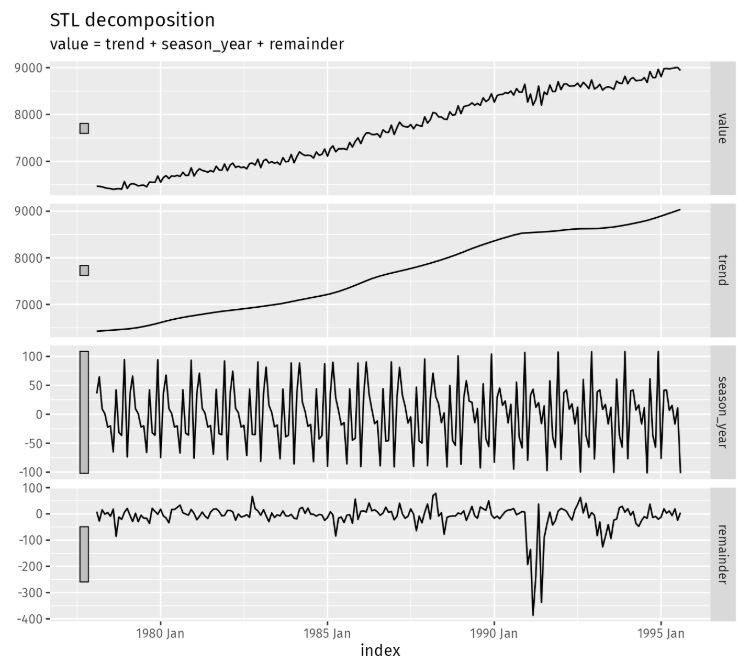
\includegraphics[keepaspectratio]{Figure3-19.png}}
\#\#\#\# Figure 3.20: Seasonal component from the decomposition shown in
the previous figure.
\pandocbounded{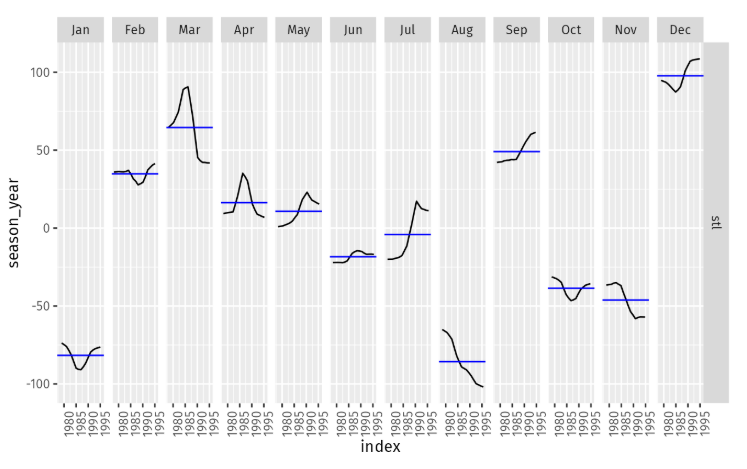
\includegraphics[keepaspectratio]{Figure3-20.png}}

\paragraph{a) Write about 3--5 sentences describing the results of the
decomposition. Pay particular attention to the scales of the graphs in
making your
interpretation.}\label{a-write-about-35-sentences-describing-the-results-of-the-decomposition.-pay-particular-attention-to-the-scales-of-the-graphs-in-making-your-interpretation.}

\paragraph{b) Is the recession of 1991/1992 visible in the estimated
components?}\label{b-is-the-recession-of-19911992-visible-in-the-estimated-components}

\end{document}
